% !TEX root = ./rosbook_jp.tex
%-------------------------------------------------------------------------------
\chapterimage{chapter_head_7.pdf}

%-------------------------------------------------------------------------------
\chapter{パッケージの導入方法}\index{パッケージの導入方法}

本章では、ROSを用いて作成され、公開されている様々なパッケージを導入する方法について説明する。ROSでは、現在まで約5,800個のパッケージが公開されており、その数はROSの普及が進むにつれて急速に増えつつある。ROSを用いれば、ロボットアプリケーションに必要な機能を、開発者がそれぞれ個別に作成する必要はない。適切なパッケージを見つける方法さえ知っていれば、世界中の開発者が既に開発したパッケージを利用でき、アプリケーション開発にかかる時間、コストを大幅に低減できる。これがROSの基本理念であり、知識や技術が蓄積されていくことで、ロボット開発が加速度的に効率化される。

%-------------------------------------------------------------------------------
\section{ロボットパッケージ}\index{ロボットパッケージ}

ロボットの構成要素はハードウェアとソフトウェアに大別される。ハードウェアには、モータ、ギア、制御回路、センサなどが含まれる。一方、ソフトウェアは、ロボットのハードウェアを制御するマイクロコントローラのファームウェアから、地図作成、ナビゲーション、動作生成、ユーザインタフェースなどの高度なアプリケーションソフトウェアまで様々である。
アプリケーションソフトウェアには、Willow GarageやClearpathのようなロボット関連企業、オープンソースロボット財団(OSRF)、大学や企業の研究室、個人の開発者により開発され、パッケージとして配布されているものもある。これらのパッケージは、ロボットに対するロボットパッケージ注1と、センサに対するセンサパッケージ注2に分類される。
ROSで用いられる代表的なロボットパッケージとしては、Willow Garageで開発されたPR2注3とWillow Garage, OSRF, Yujin Robotが共同開発したタートルボット(turtlebot)注4に対するロボットパッケージが挙げられる。PR2は、Willow Garageが研究用途に開発したヒューマノイド型ロボットであり、他のロボットパッケージは、PR2パッケージを参考に開発されているものが多い。しかし、PR2は汎用的で優れた性能をもつ一方、価格が高いという問題があった。これに対し、ロボット開発費用を抑え、低価格で提供されたロボットパッケージが移動ロボット、タートルボットである。当初、タートルボットはiRobot社のRoomba createを移動ベースとして用いていたが、その後開発されたタートルボット 2では、Yujin Robot社のKobukiが採用されている。タートルボットの詳細については、9章でタートルボットに関するロボットパッケージの使い方とともに説明する。


\begin{figure}[ht]
  \centering
  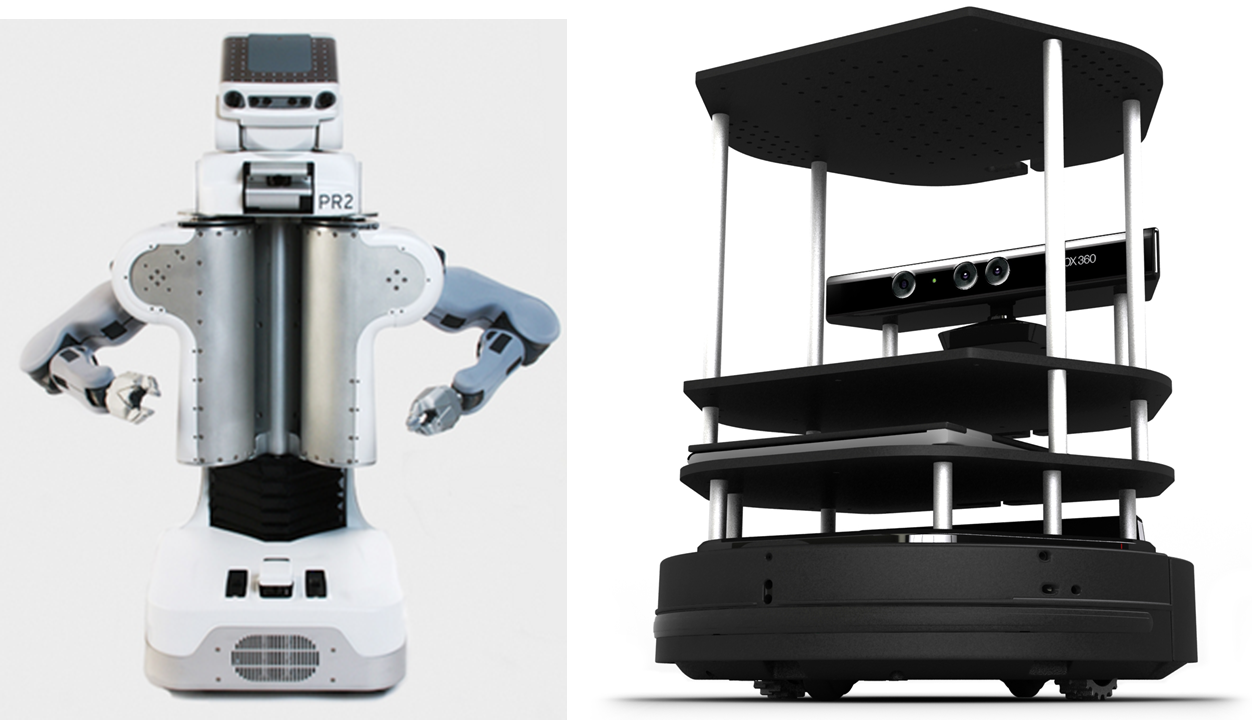
\includegraphics[width=\columnwidth]{pictures/chapter7/pic_07_01.png}
  \caption{ PR2(左)、タートルボット2(右)}
\end{figure}


この代表的な二つのロボット以外にも、ROSのWiki(http://wiki.ros.org/Robots)では、マニピュレータや移動ロボット、自動走行車、ヒューマノイドなど、140種類以上の多様なロボットパッケージが公開されている。

\begin{figure}[h]
  \centering
  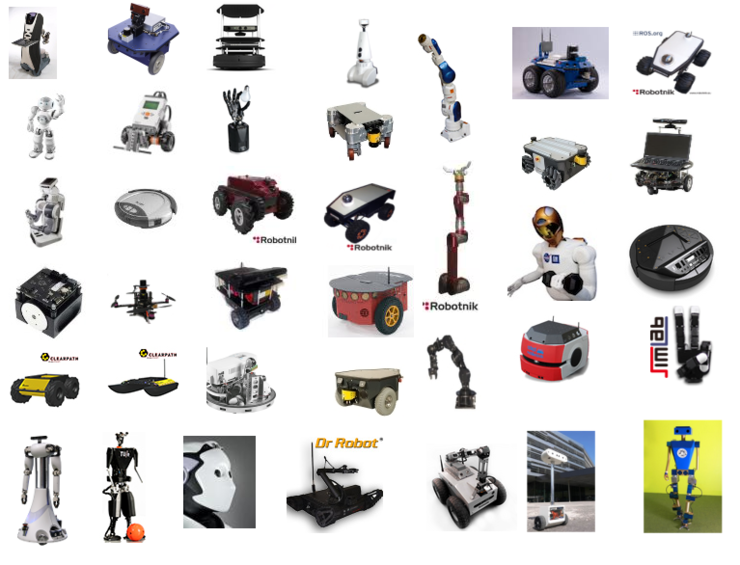
\includegraphics[width=\columnwidth]{pictures/chapter7/pic_07_02.png}
  \caption{ROSを導入したロボット(http://wiki.ros.org/Robots)}
\end{figure}

使用したいロボットパッケージが公開されているかを調べるには、ROS Wiki(http://wiki.ros.org/Robots)で確認するか、あるいは次のコマンドを実行すればいい。

\begin{lstlisting}[language=ROS]
$ apt-cache search ros-indigo
\end{lstlisting}

使用するロボットのパッケージが公式パッケージであれば、インストールは簡単である。いくつかの例を挙げてみよう。

・PR2のパッケージをインストールするコマンド
\begin{lstlisting}[language=ROS]
$ sudo apt-get install ros-indigo-pr2*
\end{lstlisting}

・タートルボット 2パッケージをインストールするコマンド
\begin{lstlisting}[language=ROS]
$ sudo apt-get install ros-indigo-turtlebot ros-indigo-turtlebot-apps ros-indigo-turtlebot-interactions ros-indigo-turtlebot-simulator ros-indigo-kobuki-ftdi
\end{lstlisting}

・Jackalロボットのパッケージをインストールするコマンド
\begin{lstlisting}[language=ROS]
$ sudo apt-get install ros-indigo-jackal-desktop
\end{lstlisting}

もし、使用したいロボットパッケージが公式には提供されていなくても、通常、そのパッケージに関するWikiでインストール方法が説明されている。例えば、有名な移動ロボットのパイオニア(Pioneer)注5は、次のようにcatkinビルドシステムのユーザーソースフォルダに移動した後、Wikiに記されているリポジトリからロボットパッケージをダウンロードすることでインストールできる。

\begin{lstlisting}[language=ROS]
$ cd ~/catkin_ws/src %*→ catkinビルドシステムのユーザーソースフォルダに移動*)
$ hg clone http://code.google.com/p/amor-ros-pkg/ %*→ ファイルをリポジトリに追加*)
\end{lstlisting}

このように、使用したいロボットパッケージが見つかれば、公開されたROS公式パッケージをインストールするか、Wikiに記述されているインストール方法を参照して、オープンソースのリポジトリからファイルをダウンロードした後、ビルドすればよい。ロボットパッケージには、ロボットの実行ノード、センサデータの取得と処理ノード、リモートコントロールのノードなどが含まれている。また、関節型ロボットのパッケージには逆運動学のノード、移動ロボットであればナビゲーションノードなども含まれる。パッケージに含まれている各ノードの仕様は、ロボットパッケージのWikiで説明されている。

%-------------------------------------------------------------------------------
\section{センサパッケージ}\index{センサパッケージ}

ロボットには多種多様なセンサが搭載されている。センサにより得られる情報は、ロボットの位置、姿勢、空間、力、画像、音声、慣性、振動、電流、RFIDなど、多岐にわたる。ROSで提供するセンサパッケージは徐々に増えつつあり、またI2CやUARTを採用したセンサはインターフェイスを統一する方向にある。センサの製造会社も積極的にROSセンサパッケージをサポートしはじめており、今後も多くのセンサがROSに対応すると思われる。

\begin{figure}[h]
  \centering
  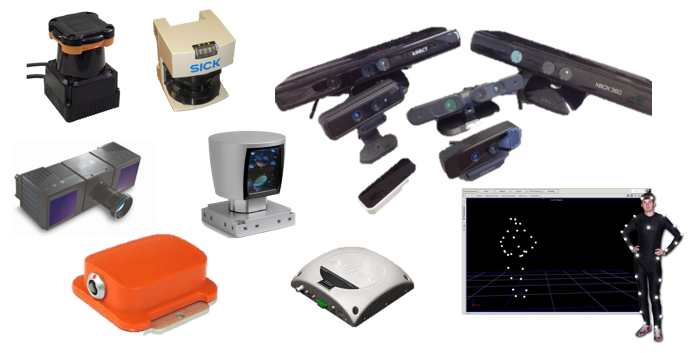
\includegraphics[width=\columnwidth]{pictures/chapter7/pic_07_03.png}
  \caption{ROSで使用可能なセンサの例}
\end{figure}

ROSのセンサパッケージの種類、使い方、ソースコードの公開情報などは、ROSのセンサ関連のWiki(http://wiki.ros.org/Sensors)にまとめられている。センサはカテゴリ区分されており、たとえば1D range finders、2D range finders、3D Sensors、Pose Estimation(GPS + IMU)、Cameras、Sensor Interfaces、Audio/Speech Recognition、Environmental、Force/Torque/Touch Sensors、Motion Capture、Power Supply、RFID等がある。
 ROSのセンサパッケージで特に重要なカテゴリを以下に示す。

\begin{itemize}
\item 1D range finders:赤外線方式の測距センサであり、主に低価格のロボットに使用される。
\item 2D range finders:いわゆるレーザレンジファインダ(Laser range finder, LRF)であり、障害物回避やSLAMに多く使用される。
\item 3D Sensors:Microsoft社のKinect、ASUS社Xtionなどの3次元計測センサである。
\item Audio/Speech Recognition:音声認識パッケージのカテゴリであるが、現在はまだ種類が少ない。
\item Cameras:物体認識、顔認識、文字認識などに使用されるカメラのドライバや各種アプリケーションパッケージを集めている。
\item Sensor Interfaces:現在はまだPCから直接情報を取得できるセンサ、およびWebプロトコルをサポートしているセンサは少なく、多くのセンサはマイクロプロセッサを介して情報を出力する。これらのセンサは、PCとマイクロプロセッサ間でUART通信を利用して情報をやり取りすることが多いが、このカテゴリでは、PC側のインターフェイスを統一し、APIとして提供している。
\end{itemize}

このように様々なセンサパッケージが公開されているので、目的に合うセンサを探して利用しよう。センサパッケージの詳しい使い方は、8章で説明する。

%-------------------------------------------------------------------------------
\section{公開パッケージの使い方}\index{公開パッケージの使い方}

ROSで公開されているパッケージは 2015年7月20日の時点でROS Indigo向けに約1,800種類(http://www.ros.org/debbuild/indigo.html)あり、これまでリリースされた全てのROSバージョンに対して、ユーザーが開発・公開したパッケージは、約5,800個(http://rosindex.github.io/stats/)に達する。この節では、公開されているなかから必要なパッケージを検索する方法、パッケージのインストールおよび使用方法について述べる。
パッケージを検索するには、まず、次のWebページにアクセスする。

http://www.ros.org/browse/list.php

図7-4のように、利用可能なパッケージの一覧がブラウザに表示されるので、Webページの上部のROSのバージョンを選択するボタンで"indigo"をクリックし、ROSのindigoバージョンのパッケージのリストを表示する。

\begin{figure}[h]
  \centering
  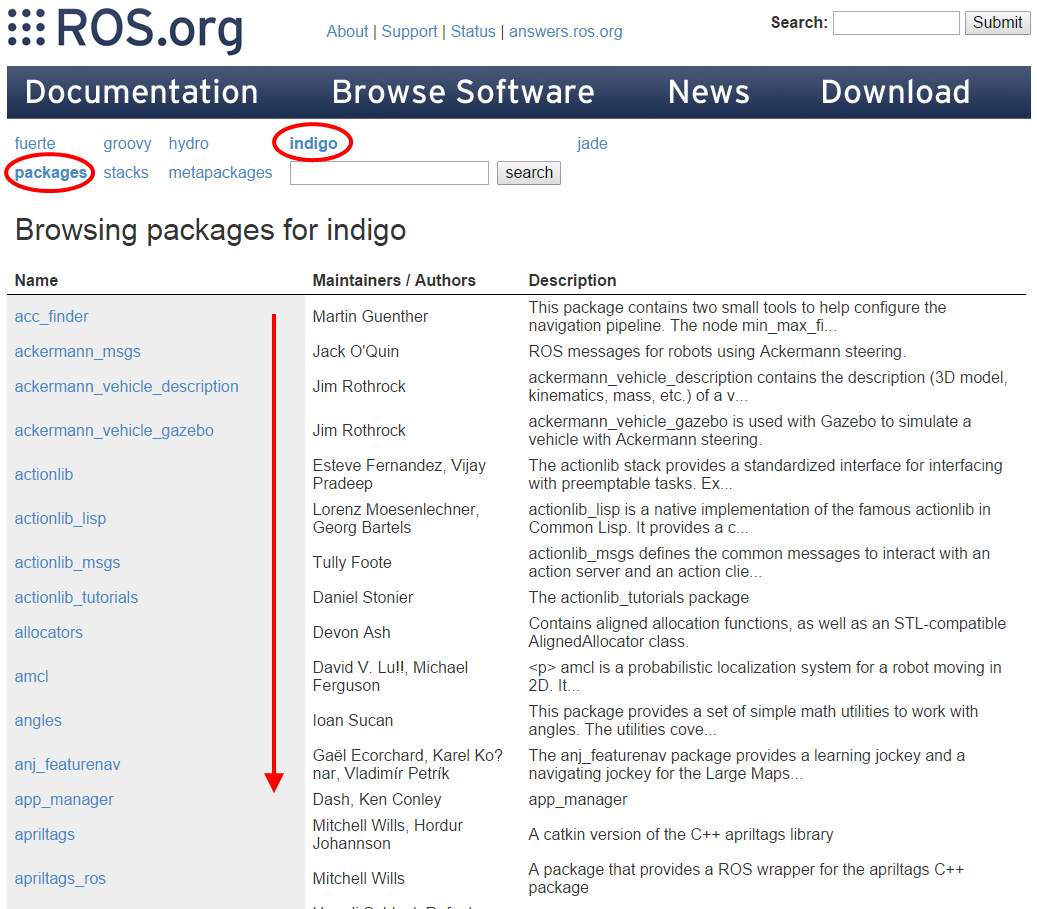
\includegraphics[width=\columnwidth]{pictures/chapter7/pic_07_04.png}
  \caption{ROSパッケージのリスト}
\end{figure}


このリストは、ROS indigoバージョン向けに公開されたパッケージの一覧である。同様に、以前のバージョンのhydro向けには1,930種類以上、最も広く使われたFuerte向けには2,720種類以上のパッケージが公開されている。パッケージのなかには、開発が継続的に行われ、定期的にバージョンアップされているものだけでなく、開発が中断され、上位のバージョンには含まれていないものもある。しかし、そのようなパッケージの多くも、若干の修正を加えることで最新バージョンのROSで利用できるようになる。
では、必要なパッケージを検索し、インストールして、実際に動作させるまでの一連の流れを、具体例を挙げて説明していく。ここでは、「USBカメラを利用して物体検出をおこなうこと」を目的としよう。

%-------------------------------------------------------------------------------
\subsection{パッケージの検索}

まず、公開されているROSパッケージから目的に合うものを検索する。以下のいずれかのページにおいて、検索キーワード「find object(物体検出)」を右上のSearch欄に入力し、Submitボタンを押す。なお、同じ検索キーワードでも1回目と2回目以降で検索範囲が異なるので、複数回試すことを推奨する。

http://wiki.ros.org/
http://www.ros.org/browse/list.php

\begin{figure}[h]
  \centering
  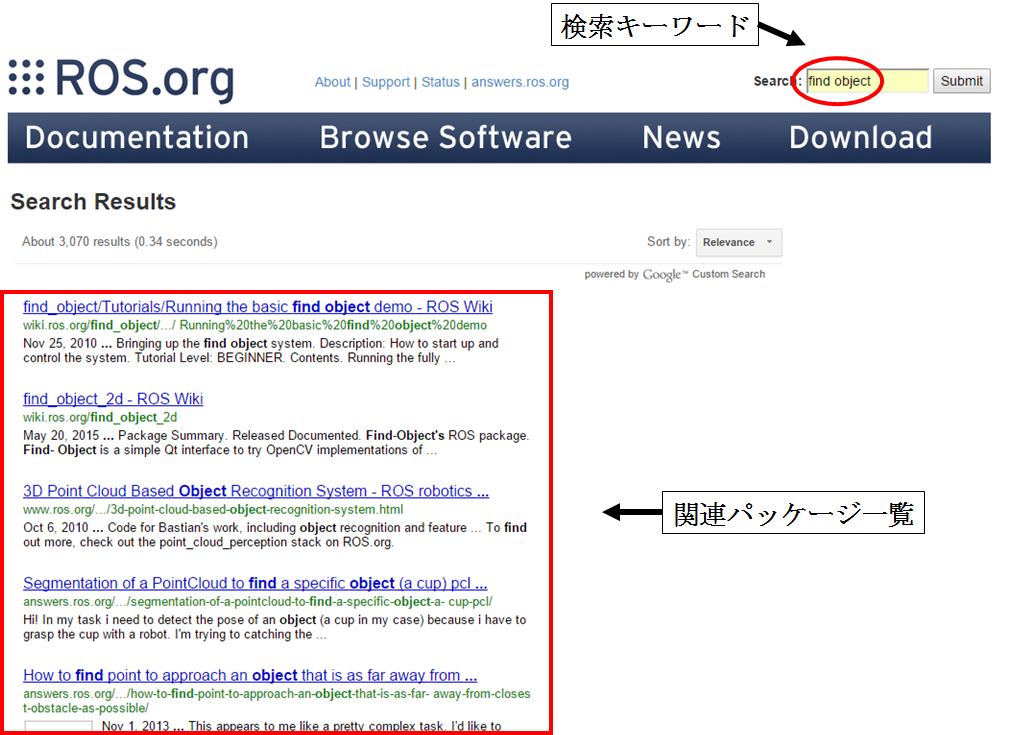
\includegraphics[width=\columnwidth]{pictures/chapter7/pic_07_05.png}
  \caption{パッケージの検索方法}
\end{figure}

検索キーワードが適切であれば、図7-5のように関連するパッケージが表示される。多数の関連パッケージがあるが、ここでは上から2つ目の「find\_object\_2d - ROS Wiki」にある「find\_object\_2d」パッケージを利用する。パッケージを導入する際には、ビルドシステムがcatkinかrosbuildか、誰が製作したものか、オープンソースのライセンスの種類などの情報を確認し、注意深く検討すべきである。
find\_object\_2dパッケージを導入するには、まず上から2つ目の「find\_object\_2d - ROS Wiki」をクリックし、図7-6に示すfind\_object\_2dパッケージのWikiページを開く。次に、上部の「Indigo」のボタンを押し、Indigoバージョンの情報を表示する。このページには、図7-6のように、パッケージのリポジトリアドレス、パッケージの依存関係(右のDependenciesをクリックすると表示される)、プロジェクトのWebページへのリンク(External website)などが記載されている。特に、パッケージの依存関係は必ず確認しよう。次項で示すように、関連パッケージは目的のパッケージより先にインストールしておく必要がある。

\begin{figure}[h]
  \centering
  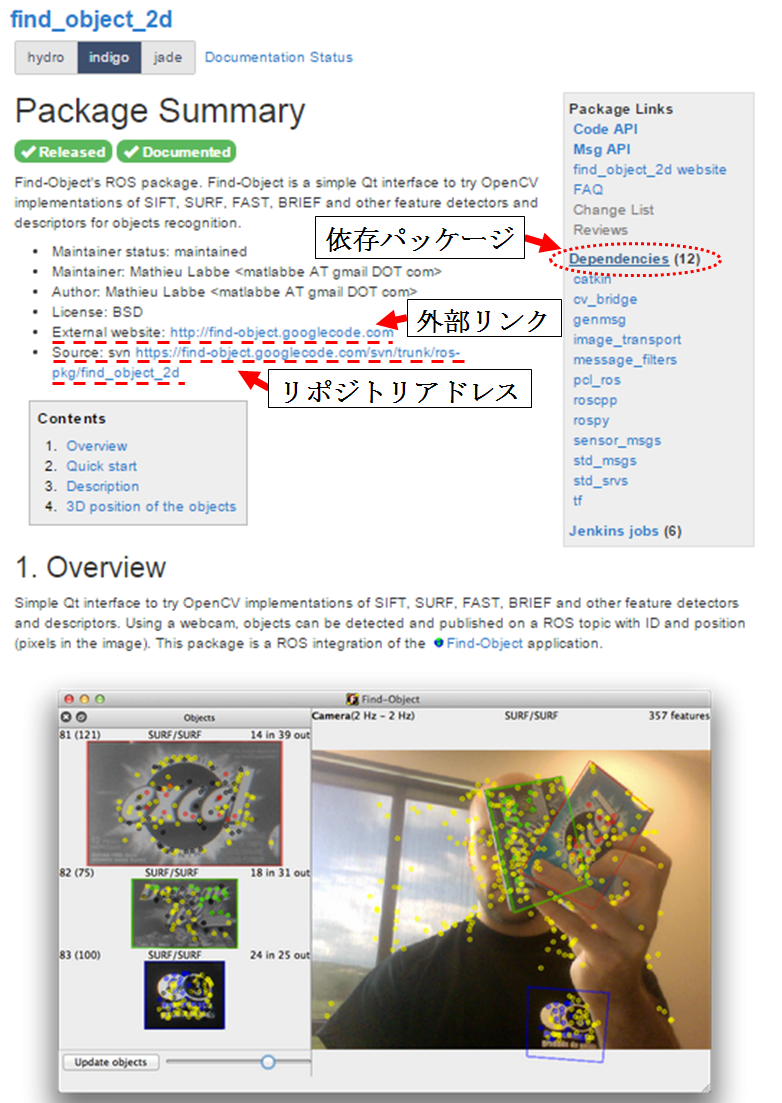
\includegraphics[width=\columnwidth]{pictures/chapter7/pic_07_06.png}
  \caption{パッケージ情報}
\end{figure}

%-------------------------------------------------------------------------------
\subsection{依存パッケージのインストール}

find\_object\_2dパッケージのWikiページ(http://wiki.ros.org/find\_object\_2d)でパッケージの依存関係(Dependencies)を確認すると、このパッケージには12種類のパッケージが必要であることがわかる。

\begin{itemize}
\item catkin
\item cv\_bridge
\item genmsg
\item image\_transport
\item message\_filters
\item pcl\_ros
\item roscpp
\item rospy
\item sensor\_msgs
\item std\_msgs
\item std\_srvs
\item tf
\end{itemize}

rospack listコマンド、あるいはrospack findコマンドで、上記の必要なパッケージが既にインストールされているかを確認する。

・rospack listコマンドによる確認
\begin{lstlisting}[language=ROS]
$ rospack list
actionlib /opt/ros/indigo/share/actionlib
actionlib_msgs /opt/ros/indigo/share/actionlib_msgs
actionlib_tutorials /opt/ros/indigo/share/actionlib_tutorials
...
%*(出力されたリストに必要なパッケージが含まれているかを確認)*)
\end{lstlisting}

rospack findコマンドによる確認(インストールされている場合)

\begin{lstlisting}[language=ROS]
$ rospack find cv_bridge
/opt/ros/indigo/share/cv_bridge
\end{lstlisting}

rospack findコマンドによる確認(インストールされていない場合)

\begin{lstlisting}[language=ROS]
$ rospack find cv_bridge
 [rospack] Error: package 'cv_bridge' not found
\end{lstlisting}

インストールされていない場合には、それぞれのWikiページでインストール方法を確認し、以下のようにインストールする。

\begin{lstlisting}[language=ROS]
$ sudo apt-get install ros-indigo-cv-bridge
\end{lstlisting}

また、Wikiページ(http://wiki.ros.org/find\_object\_2d)の「2. Quick start」には、find\_object\_2dパッケージではuvc\_cameraパッケージ(http://wiki.ros.org/uvc\_camera)を利用することが記述されている。そこで、uvc\_cameraパッケージをインストールする。

\begin{lstlisting}[language=ROS]
$ sudo apt-get install ros-indigo-uvc-camera
\end{lstlisting}

%-------------------------------------------------------------------------------
\subsection{パッケージのインストール}

全ての依存パッケージをインストールした後、find\_object\_2dパッケージをインストールする。図7-6には、パッケージの入手先であるリポジトリアドレスが、以下のように記載されている。

Source: svn https://find-object.googlecode.com/svn/trunk/ros-pkg/find\_object\_2d

この方法では、インストールされたパッケージに含まれるソースファイルを、自分でコンパイルする必要がある。しかし、あらかじめコンパイルされたファイル(バイナリファイル)を利用し、より手軽にパッケージを導入する方法もある。以下では、その手順を紹介する。

まず、パッケージについてより詳しく調べるために、External websiteに記されたアドレス「http://find-object.googlecode.com」をクリックすると、そのページが「http://introlab.github.io/find-object/」に移動していると表示されるので、再度「http://introlab.github.io/find-object/」をクリックする。このページの中程に「Install」の項があり、そこにROSのインストール方法を記したGitHubへのリンク「See find\_object\_2d on GitHub.」(図7-7)があるので、それをクリックして「https://github.com/introlab/find-object/tree/master#find\_object\_2d-ros-package」に移動する(図7-8)。

\begin{figure}[h]
  \centering
  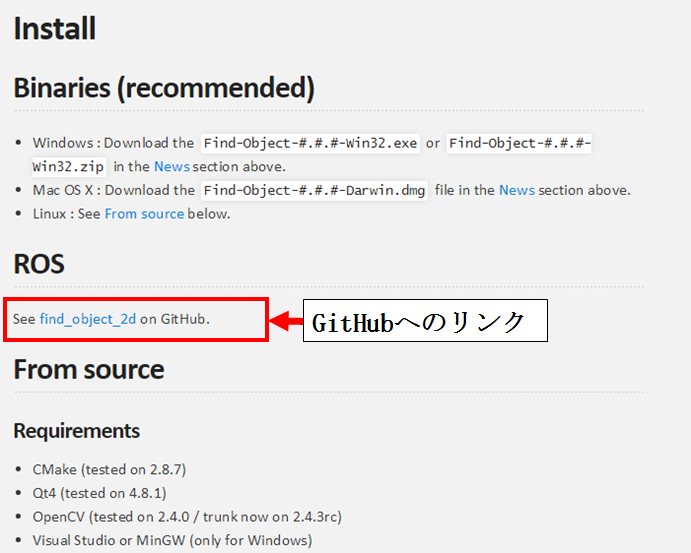
\includegraphics[width=\columnwidth]{pictures/chapter7/pic_07_07.png}
  \caption{GitHubへのリンク}
\end{figure}

\begin{figure}[h]
  \centering
  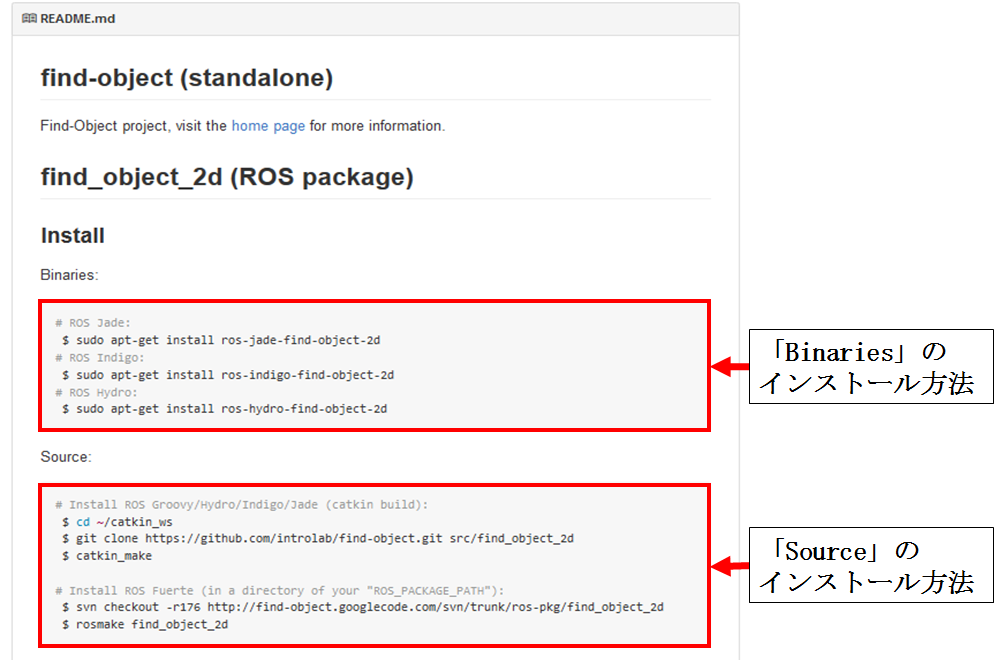
\includegraphics[width=\columnwidth]{pictures/chapter7/pic_07_08.png}
  \caption{インストール方法を記したWebページ}
\end{figure}

ここにはコンパイル済みのパッケージ「Binaries」のインストール方法、あるいは自分でコンパイルする必要のある「Source」のインストール方法が記載されている。ここでは、コンパイル済みのパッケージ「Binaries」をインストールする。

\begin{lstlisting}[language=ROS]
$ sudo apt-get install ros-indigo-find-object-2d
\end{lstlisting}

なお、このパッケージはROSとは直接関係のないOpenCVとQtのライブラリを使用している。これらをインストールしていない場合には、事前に以下のようにインストールしておく必要がある。

\begin{lstlisting}[language=ROS]
$ sudo apt-get install libopencv-dev // %*OpenCVのインストール*)
$ sudo apt-get install libqt4-dev    // %*Qtのインストール*)
\end{lstlisting}

以上により、物体検出に必要なすべてのパッケージをインストールできた。もし、これ以外に依存パッケージで問題が生じた場合、opencv2、openni\_camera、ros2opencvなどがインストールされているかを確認してほしい。

%-------------------------------------------------------------------------------
\subsection{パッケージのノードの実行}

find\_object\_2dパッケージのWikiページ(http://wiki.ros.org/find\_object\_2d#Quick\_start)の記述に従って、パッケージを実行する。まず、roscoreを起動して、別のターミナルウィンドウを開き、次のコマンドでカメラのノードを起動しよう。

\begin{lstlisting}[language=ROS]
$ roscore
$ rosrun uvc_camera uvc_camera_node
\end{lstlisting}

次に、別のターミナルウィンドウを開き、以下のコマンドで物体検出ノードを実行する。

\begin{lstlisting}[language=ROS]
$ rosrun find_object_2d find_object_2d image:=image_raw
\end{lstlisting}

検出対象の画像をPNG形式やJPEG形式など一般的な画像ファイル形式で保存しておき、起動したアプリケーション上にそのファイルをドラッグ・アンド・ドロップする。ここでは、検出対象として、以下の2枚の画像を使用する。

\begin{figure}[h]
  \centering
  
\includegraphics[width=\columnwidth]{pictures/chapter7/pic_07_09.png}
  \caption{検出対象(「find\_object_2d」および「ROS.org」と書かれた画像)}
\end{figure}

それでは、実際に物体検出に挑戦してみよう。図7-10のように、検出対象の画像を含む絵を用意し、それを紙に印刷したものをカメラで撮影する。実行結果の例を図7-10に示す。図7-9に示した2つの文字列が四角で囲まれ、適切に検出されている。なお、ターミナルウィンドウで、「rostopic echo /object」と入力すると、検出された対象の座標値が出力される。このパッケージを利用して新たなパッケージを作成する際には、この座標値をトピックで受信して利用することができる。

以上で公開されているパッケージの活用方法の一例を示した。ROS Wiki(http://wiki.ros.org/)には、パッケージの開発者によって、パッケージの使用方法が詳細に記述されているので、公開パッケージの使用の際には参考にしてほしい。

\begin{figure}[h]
  \centering
  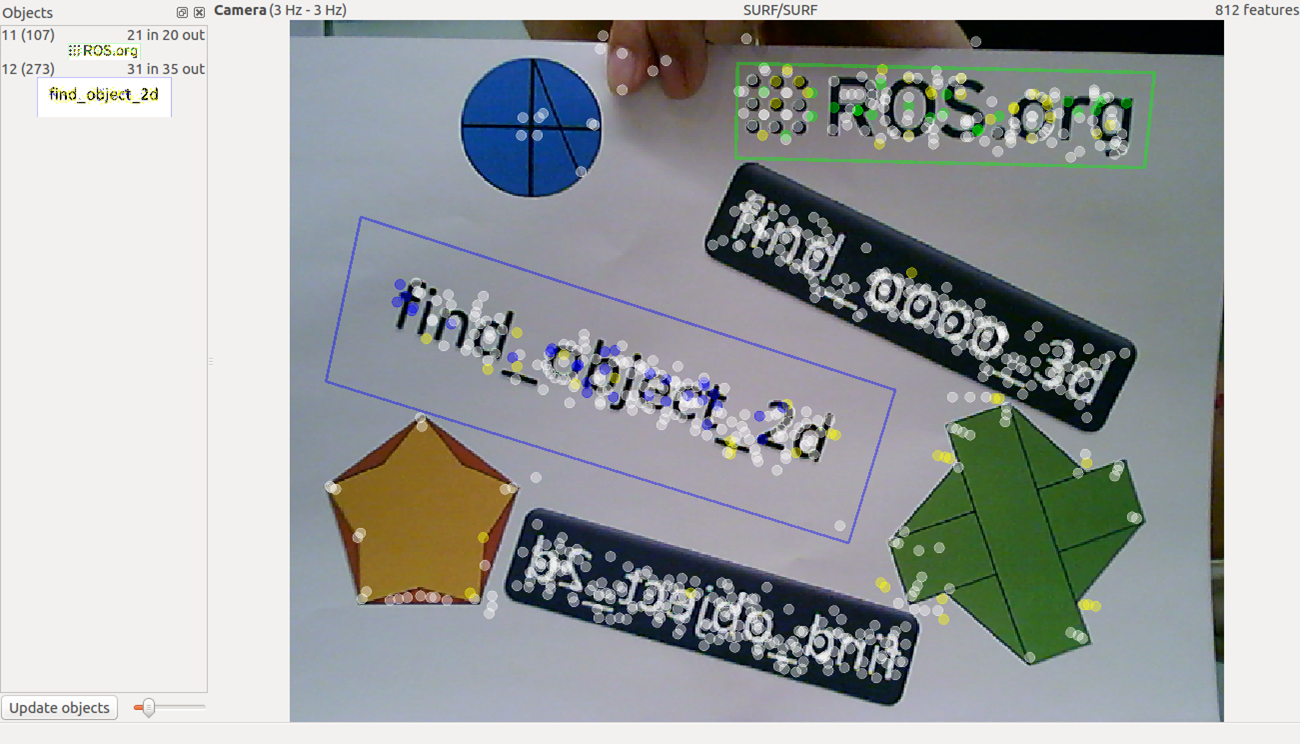
\includegraphics[width=\columnwidth]{pictures/chapter7/pic_07_10.png}
  \caption{画像の検出結果}
\end{figure}


% 注1  http://wiki.ros.org/Robots
% 注2  http://wiki.ros.org/Sensors
% 注3  http://wiki.ros.org/Robots/PR2
% 注4  http://wiki.ros.org/Robots/TurtleBot
% 注5  http://wiki.ros.org/ROSARIA



%-------------------------------------------------------------------------------
